\section{Experiment 3: Adding Semantic Noise}

% Corresponding Progress Reports
% https://www.notion.so/241025-Matthias-Exploration-of-adversarial-augmentation-199ccb0746f74fd696b8bebe8590fe15
% https://www.notion.so/241101-Matthias-Using-Adversarial-perturbation-to-augment-clip-vision-input-in-brain-diffuser-3e8235a27e3c4f4eb67f61a467fd5ada
% https://www.notion.so/241108-Matthias-further-exploration-of-perturbations-196925e9c9b94c04be7a7d1891ce5389?pvs=23
% https://www.notion.so/241114-matthias-brain-diffuser-perturbation-big-analysis-13cb45eff9104ae1929522dcf1d39bb9?pvs=23

% How to execute the whole advpert process?
% 1. Execute multi_process_pert_generation.py (it will generate perturbations for all conditions)
% 2. Execute re_recon_main.py (it will do the reconstructions for all cases -> make sure all data is ready before, baseline needs to be computed beforehand)
% 3. Execute quantitative_eval.py (extracts the quantitative measures from all predicted features/imates)
% 4. Execute create_dfs_advpert.py (creates the dataframes to evaluate the results)
% 5. Execute the analysis_advpert.py (generates the plots)
% 6. For the additional validation plots, execute clip_module_testing.py


\subsection{Background}

\subsection{Methods}

The perturbation procedure is described below. The training images are to be manipulated in such a way that they look almost the same, but the semantic information that the clipvision encoder reads from them is greatly altered. Two different algorithms are analysed to generate the perturbations in the images. It is then determined which of the two algorithms is better at achieving the goal of keeping the input image visually as close to the original as possible while at the same time producing different clipvision embeddings. Subsequently, all training data is perturbed using this algorithm and the perturbed versions are used to train the clipvision translator of the brain diffuser algorithm.

\subsubsection{Perturbation Process}

% FGSM Algorithm Formula
First, the Fast Gradient Sign Method\cite{goodfellowExplainingHarnessingAdversarial2014} (FGSM) is used to generate the perturbations. In FGSM, an image is first encoded with a model (here the clipvision encoder) in a forward step, then a loss to a desired output vector (the perturbation vector is calculated with respect to the input image , then the sign of the gradient (multiplied by a freely chosen factor $\epsilon$) is subtracted from the input image in a single backpropagation step. This procedure ensures that the clipvision output of the perturbed image is more similar to the perturbation vector. The mathematical description of the algorithm is as follows

\[
x' = x + \epsilon \cdot \text{sign}(\nabla_x J(\theta, x, y))
\]

where:
\begin{itemize}
    \item \( x' \) is the perturbed image,
    \item \( x \) is the original image,
    \item \( y \) is the perturbation vector,
    \item \( \epsilon \) is the perturbation factor,
    \item \( \nabla_x J(\theta, x, y) \) is the gradient of the loss function \( J \) w.r.t.\ \( x \),
    \item \( \text{sign}(\cdot) \) is the element-wise sign function.
    \item \( \theta \) represents the model parameters,
\end{itemize}

In principle, all possible vectors that have the same output format as the clipvision encoder can be used as perturbation vectors. In our case, we take advantage of the multimodality of the clip model and can use cliptext embeddings as perturbation vectors. In this way, the semantic information from the captions can be partially stored in the images, at best without being highly visible in the images. In our case, two types of captions are inserted into the images via the perturbation: on the one hand, captions are used that represent the valid image in question (e.g.\ a caption describing the bat for an image of a bat). On the other hand, invalid captions are used, i.e.\ where the caption describes something other than what can be seen in the image. The perturbations with valid captions will be referred to as `friendly perturbations', the perturbations with invalid captions as `adversarial perturbations'.

% IC Algorithm Formula
In addition to the one-step FGSM algorithm, an iterative perturbation method developed for this work is used. The method will be called Iterative Criterion (IC) Here, too, the input image is systematically adjusted by backpropagation so that the output of the clipvision model of the perturbed input image approach a previously selected perturbation vector. As before, this perturbation vector must be in the same space as in the FGSM algorithm, and again cliptext embeddings of friendly and adversarial captions are used. The difference to the FGSM algorithm is that the perturbation is not performed in a single step, but iteratively in several steps until a criterion is reached. The criterion determines how similar (measured by cosine distance) the output of the clipvision embedding of the perturbed image should be to the perturbation vector in comparison to the original image. For example, with a criterion of 50/50, the input image would be perturbed until the clipvision embeddings of the perturbed version have the same cosine distance from the perturbation vector as the original clipvision embeddings (with a criterion of 10/90, until the distance of the perturbed embeddings from the perturbation vector is greater than 11.1\% of the distance of the perturbed embeddings from the original embeddings). In addition, a maximum number of steps is introduced if the algorithm does not reach the target criterion. The formal definition of the algorithm is as follows 

\[
\begin{aligned}
& \textbf{Iteration: For } t = 0 \text{ to steps:}\\
& \quad 1.\; \mathbf{v}_t = \mathrm{clipvision.encode}(\mathbf{x}_t), \\[4pt]
& \quad 2.\; \ell(\mathbf{x}_t) 
\;=\; \cos\bigl(\mathbf{v}_t,\;\mathbf{v}_c\bigr), \\[4pt]
& \quad 3.\; \mathbf{x}_{t+1} 
\;=\; \mathbf{x}_t \;-\; \eta \,\nabla_{x_t} (\theta, x_t, v_c), \\[4pt]
& \quad 4.\; d_{\text{init}} 
\;=\; \cos\bigl(\mathbf{v}_t,\;\mathbf{v}_0\bigr), \\[4pt]
& \quad 5.\; \textbf{if} \;\frac{d_{\text{init}}}{\ell(\mathbf{x}_t)} 
\;>\; LC, \;\textbf{then break}.\\[6pt]
%
& \textbf{Output: } \mathbf{x}_t \quad \text{(perturbed image)}.
\end{aligned}
\]

where:
\begin{itemize}
    \item $\mathbf{x}_0$ is the original input image
    \item $\eta$ is the learning rate
    \item $LC$ is the stop criterion (number between 0 and 1)
    \item $v_0$ is the clipvision encoding of $x_0$
    \item $v_c$ is the cliptext encoding of the selected caption
    \item cos is the cosine distance
    \item steps is the maximum number of steps to iterate
\end{itemize}

For faster convergence, the learning rate is set to 3 in the first 100 steps, to 1.5 between step 100 and step 300 and then to 1. The maximum number of steps is set to 500.

\subsubsection{Perturbation Validation}

In the following, the two perturbation methods will be examined more closely, and it will be determined how well they perform in generating highly modified clipvision embeddings from a largely visually unchanged image. First, however, we will check whether the distinction between friendly and adversarial captions in terms of similarity to the input images works at all. For this purpose, the cosine distance to a friendly and a adversarial caption was measured for all 1200 input images. The results are shown in Figure~\ref{fig:advpert_sanity_check_friendly_vs_adversarial_cap}.

% Image from smith clip_module_testing.py
\begin{figure}[ht]
    \centering
    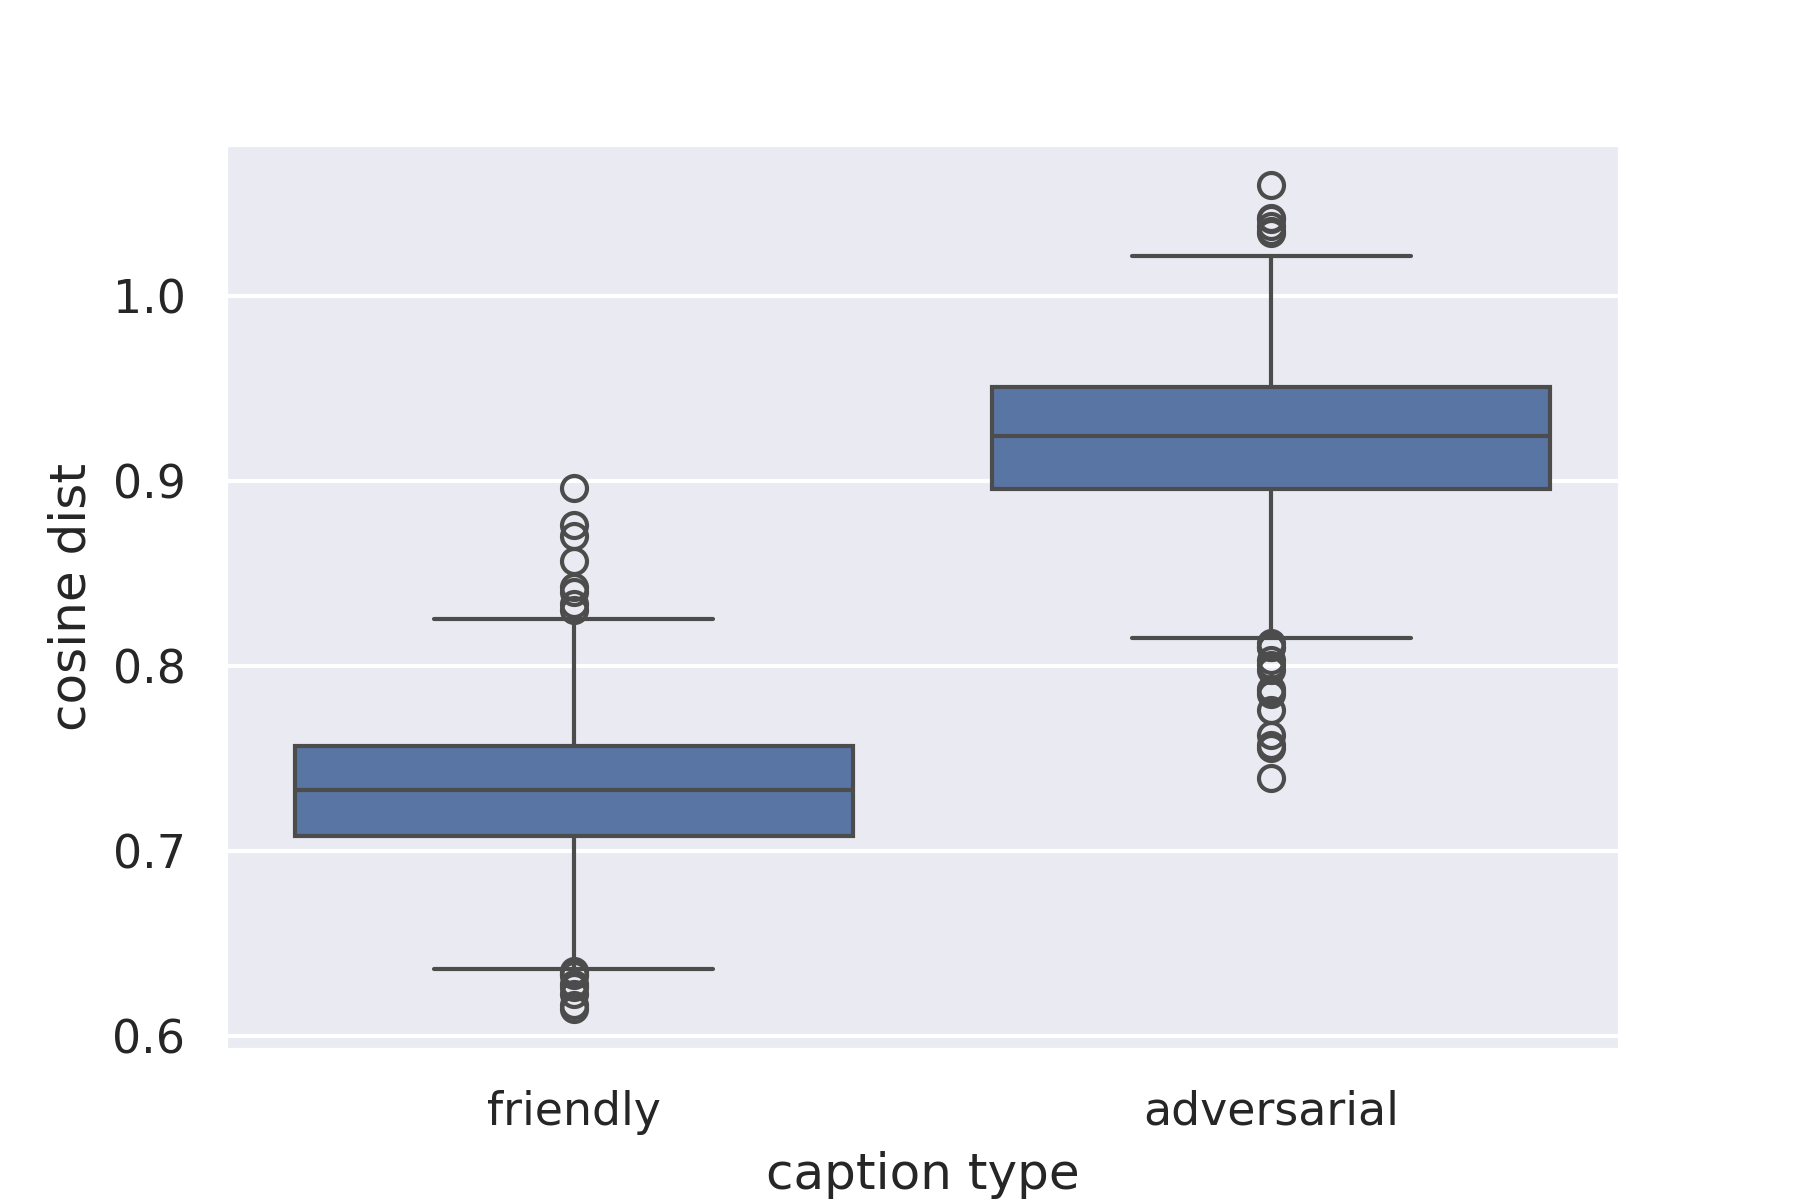
\includegraphics[width=0.6\textwidth]{plots/advpert_sanity_check_friendly_vs_adversarial_cap.png}
    \caption{A nice image}\label{fig:advpert_sanity_check_friendly_vs_adversarial_cap}
\end{figure}
% TODO: Describe the image
% -> Shows, that the corresponding captions are actually closer to the images than the other ones.
% Conclusion: I can do things like friendly and adversarial perturbations

It is clear that the friendly captions have on average a lower cosine distance to the images (0.74) than the adversarial captions (0.91). It can therefore be assumed that friendly captions are more similar to the respective images than adversarial captions. 

In the following, the IC algorithm is examined in detail in a preliminary investigation to determine whether it can achieve the goal of significantly changing the clipvision embeddings while maintaining visually similar images. For this purpose, each of the 1200 input images was perturbed with as many steps until the 50/50 criterion was reached (i.e. the cosine distance of the clipvision embeddings to the original image is exactly the same as to the cliptext embeddings of the perturbed caption). Additionally, the pixel correlation of the perturbed image to the original image was calculated for each iteration step. The average within a step was calculated for all 1200 input images. The results of this analysis are shown in Figure~\ref{fig:advpert_validation_ic_loss_curves}. 


% Show how the loss is developing for the IC criterion 
% TODO: need an image for that
% Both friendly and adversarial in one image -> To show, that both of them develop similarly
\begin{figure}[ht]
    \centering
    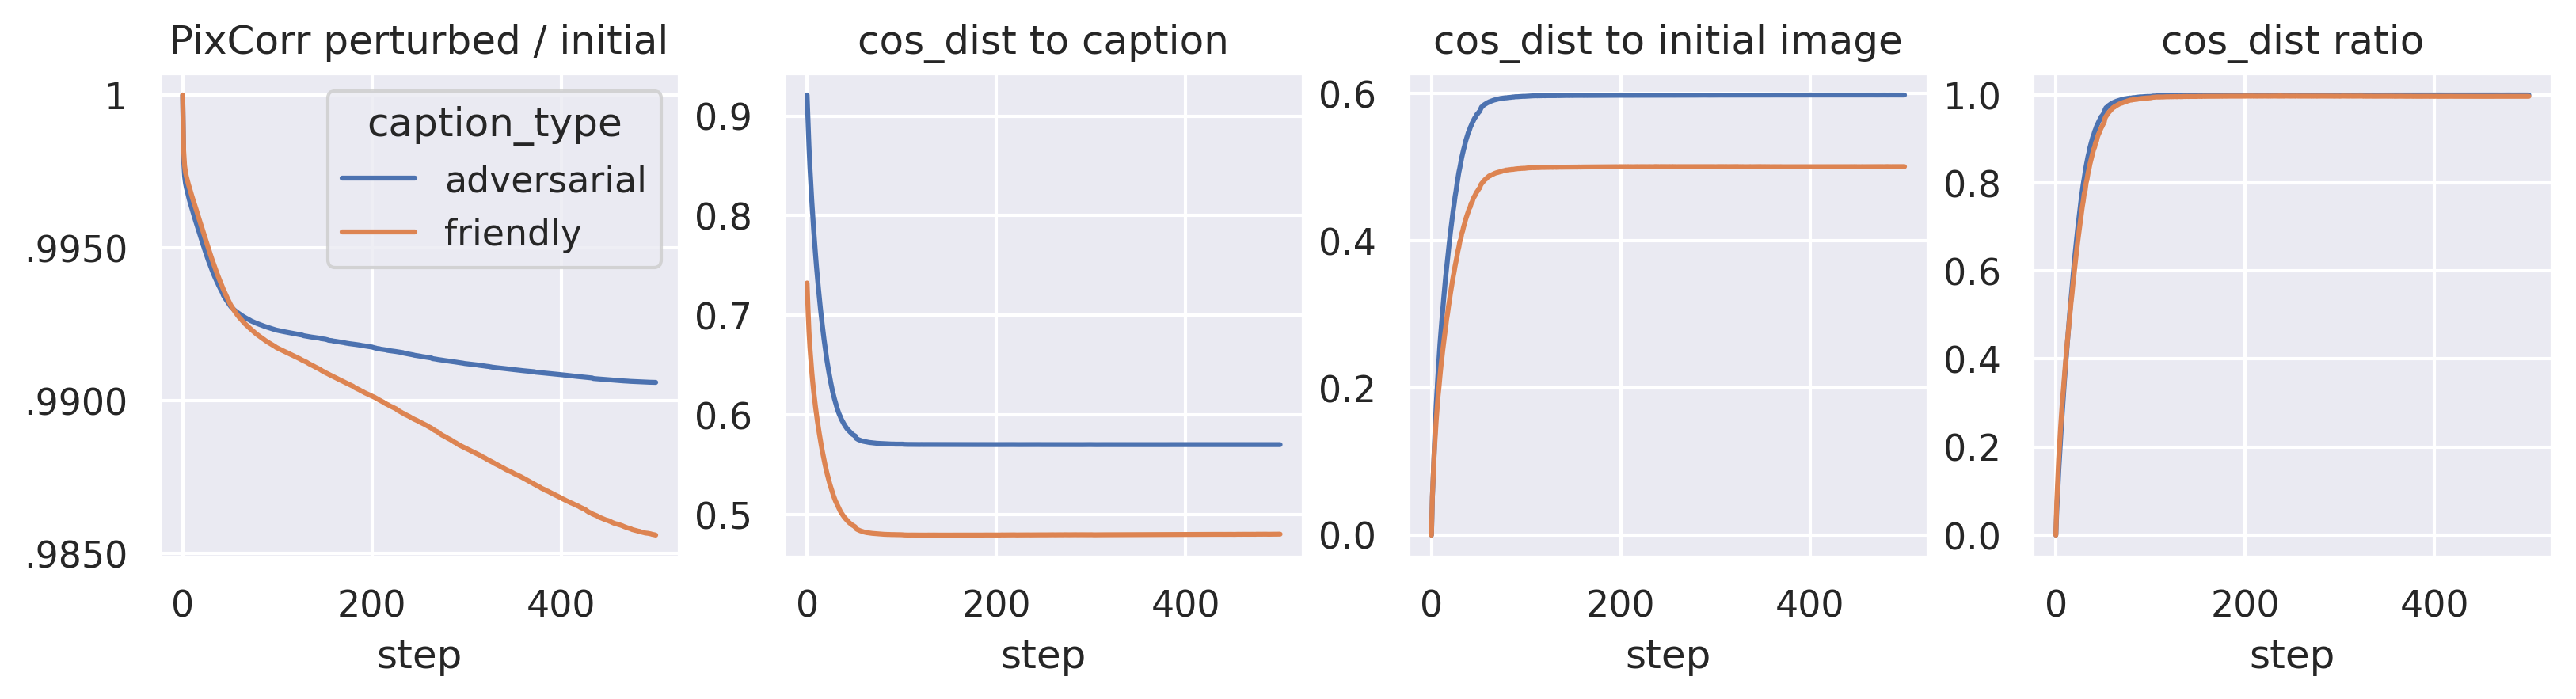
\includegraphics[width=1\textwidth]{plots/advpert_validation_ic_loss_curves.png}
    \caption{A nice image}\label{fig:advpert_validation_ic_loss_curves}
\end{figure}

The figure shows that the development for adversarial and friendly captions is comparatively similar. The pixel correlation remains very high over time, indicating a relatively small visual deviation from the original image. The cos distance to the perturbation caption decreases continuously with the number of steps, while the cos distance to the original image increases. It can be seen that the cos dist ratio has reached the 50/50 (1) criterion for most images after about 100 steps. As shown before, the initial cos distance of the original images is higher for the adversarial captions than for the friendly captions.

% Show how the results of IC change with more and more epochs (together with the IC loss plot)
    % With images for each epoch

\begin{figure}[ht]
    \centering
    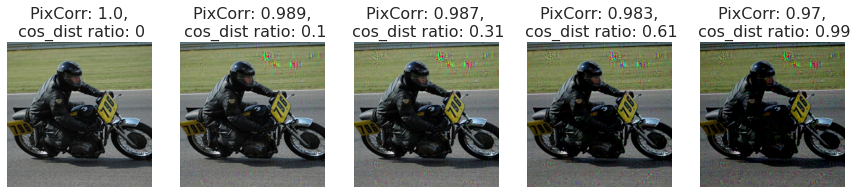
\includegraphics[width=1\textwidth]{plots/advpert_ic_qual_validation_evolution.png}
    \caption{A nice image}\label{fig:advpert_ic_qual_validation_evolution}
\end{figure}

Figure~\ref{fig:advpert_ic_qual_validation_evolution} shows a qualitative representation of how the images change during the perturbation process. It shows the respective pixel correlation to the original image (far left) and the loss ratio (synonymous with the cos dist ratio from the previous plot). It can be seen that the IC algorithm produces very local perturbations. The majority of the image remains largely untouched, but visual artefacts appear locally. In general, the IC algorithm also seems to have a bias that reduces the brightness of the image if too many perturbation steps are made. Care should therefore be taken in the final experiment not to choose too many perturbation steps in order to maintain the high pixel correlation with the original image. In summary, the IC algorithm is well suited to specifically modify the clipvision embeddings of an image, while the optical alteration, as measured by the pixel correlation, remains comparatively small. In consideration of the analysis of the IC algorithm, the criterion is set to \textbf{80/20} for further experiments. This ensures on the one hand that the perturbation has a noticeable effect on the perturbed images and approaches the cliptext embeddings of the selected captions, and on the other hand that the visual perturbation does not become too strong. 


\begin{figure}[ht]
    \centering
    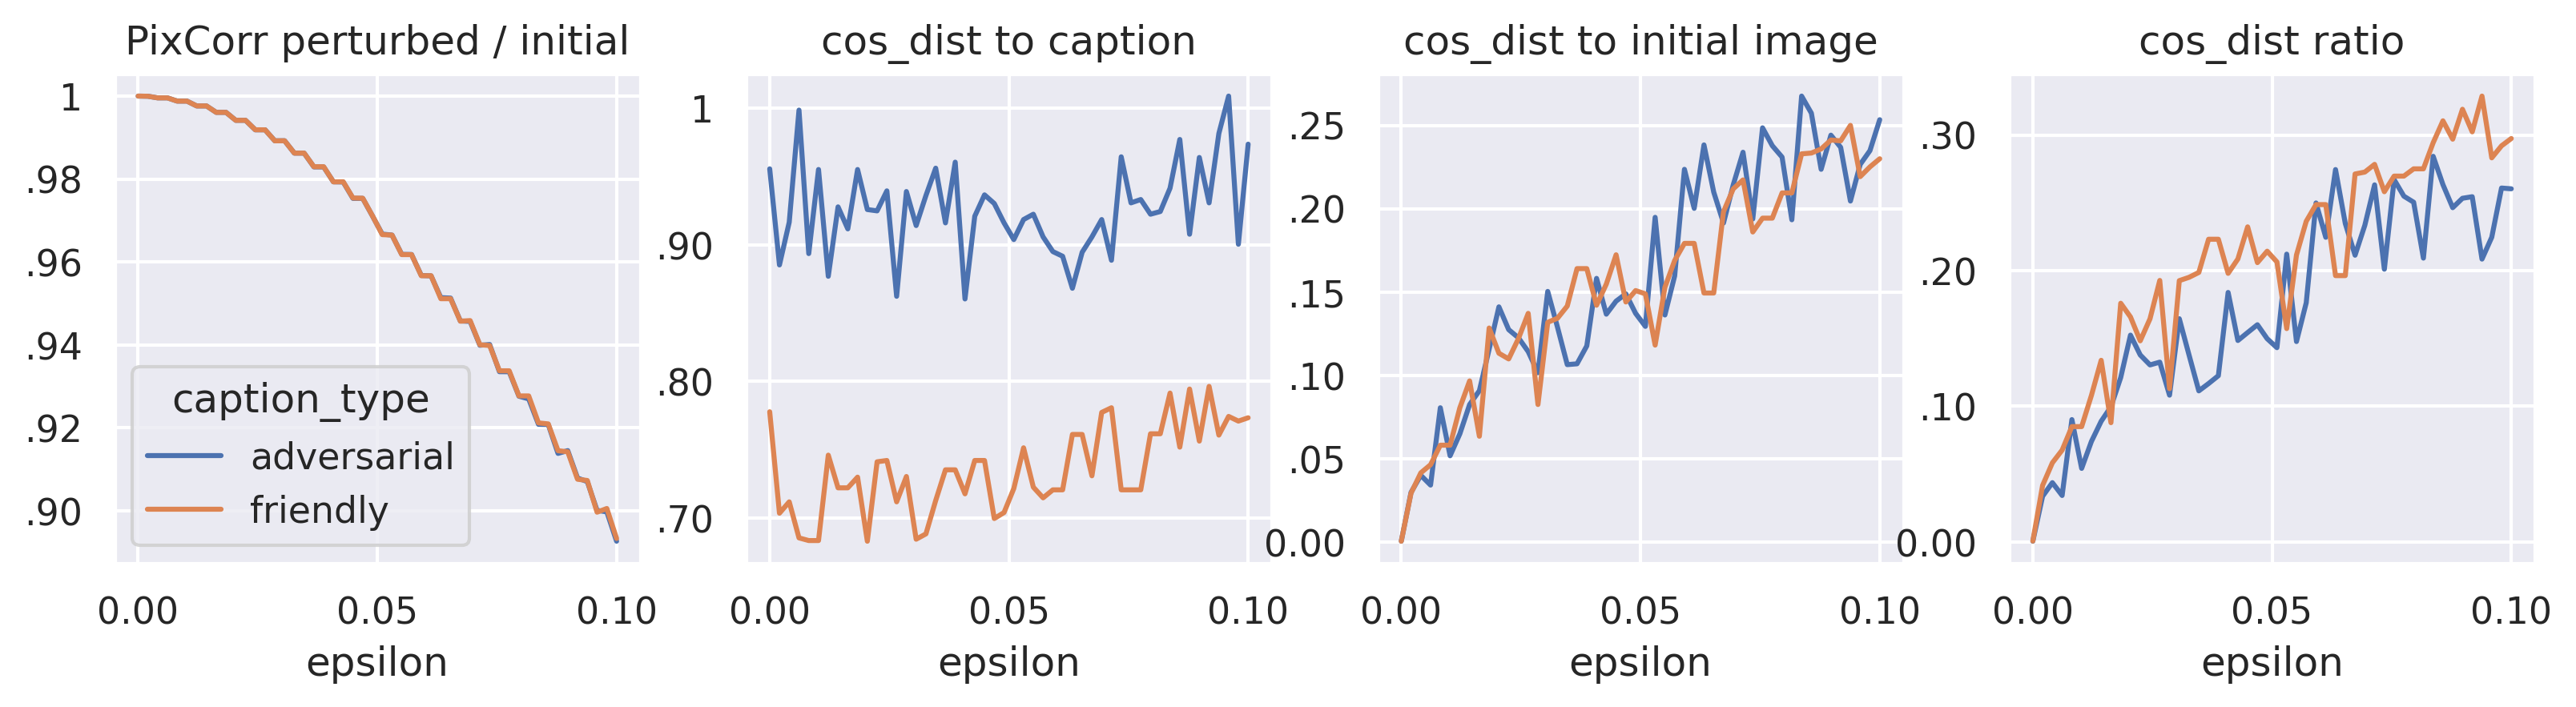
\includegraphics[width=1\textwidth]{plots/advpert_validation_fgsm_loss_curves.png}
    \caption{A nice image}\label{fig:advpert_validation_fgsm_loss_curves}
\end{figure}

FGSM is evaluated in the same way as the IC algorithm. Figure~\ref{fig:advpert_validation_fgsm_loss_curves} shows the same metrics as for IC. This time the x-axis shows not the iteration steps but the parameter epsilon, which influences how much the image may be changed in the single perturbation step. Since the FGSM algorithm always changes each pixel by the same value (with a different sign), the pixel change in the image must be exactly the same for the same epsilon (this is indicated by the same pixelCorrelation for both caption types). However, the cosine distance to the perturbation vector (caption) shows that FGSM is not able to approach the desired perturbation vector with increasing epsilon. It can be assumed that the changes here become too large to go in a specific direction. At least the distance to the original image increases with increasing epsilon, so that the increasing cos dist ratio with increasing epsilon depends only on the distance to the original image, but not on the proximity to the desired perturbation vector. 

% Show the influence of friendly vs adversarial perturbation on PixCorr
    % Both for FGSM and for IC
    % -> Not so much changes in the images
    \begin{figure}[ht]
        \centering
        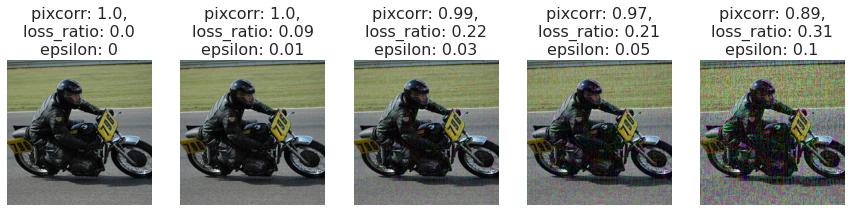
\includegraphics[width=1\textwidth]{plots/advpert_fgsm_qual_validation_evolution.png}
        \caption{A nice image}\label{fig:advpert_fgsm_qual_validation_evolution}
    \end{figure}
    

A qualitative examination of the FGSM results in Figure~\ref{fig:advpert_fgsm_qual_validation_evolution} also shows the difference to the IC algorithm: in contrast to IC, the perturbation is globally visible in the form of noise in the entire image. Local artefacts as in IC are not visible here. In summary, the FGSM algorithm is good at visually changing the image to a predictable extent, but not particularly good at making the perturbation run in a targeted direction. The perturbations here are global and are particularly noticeable as the distance from the original image increases. For further experiments the epsilon is set to \textbf{0.03}. Since a further convergence to the perturbation vectors with an increased epsilon is not to be expected with FGSM, the epsilon is chosen here so that the perturbation has an influence on the image, but does not change the original image too much.

% Define the parameters that will be used in the final test 
    % 80/10 for IC and 0.03 for FGSM

% Show how loss to original clipfeatures and caption clip features are on average for the chosen perturbations
    % Don't need to show ALL the pictures here I guess? Otherwise I'd have to do the whole perturbation process again
    % oh boy. Oh you poor little boy...
\begin{figure}[ht]
    \centering
    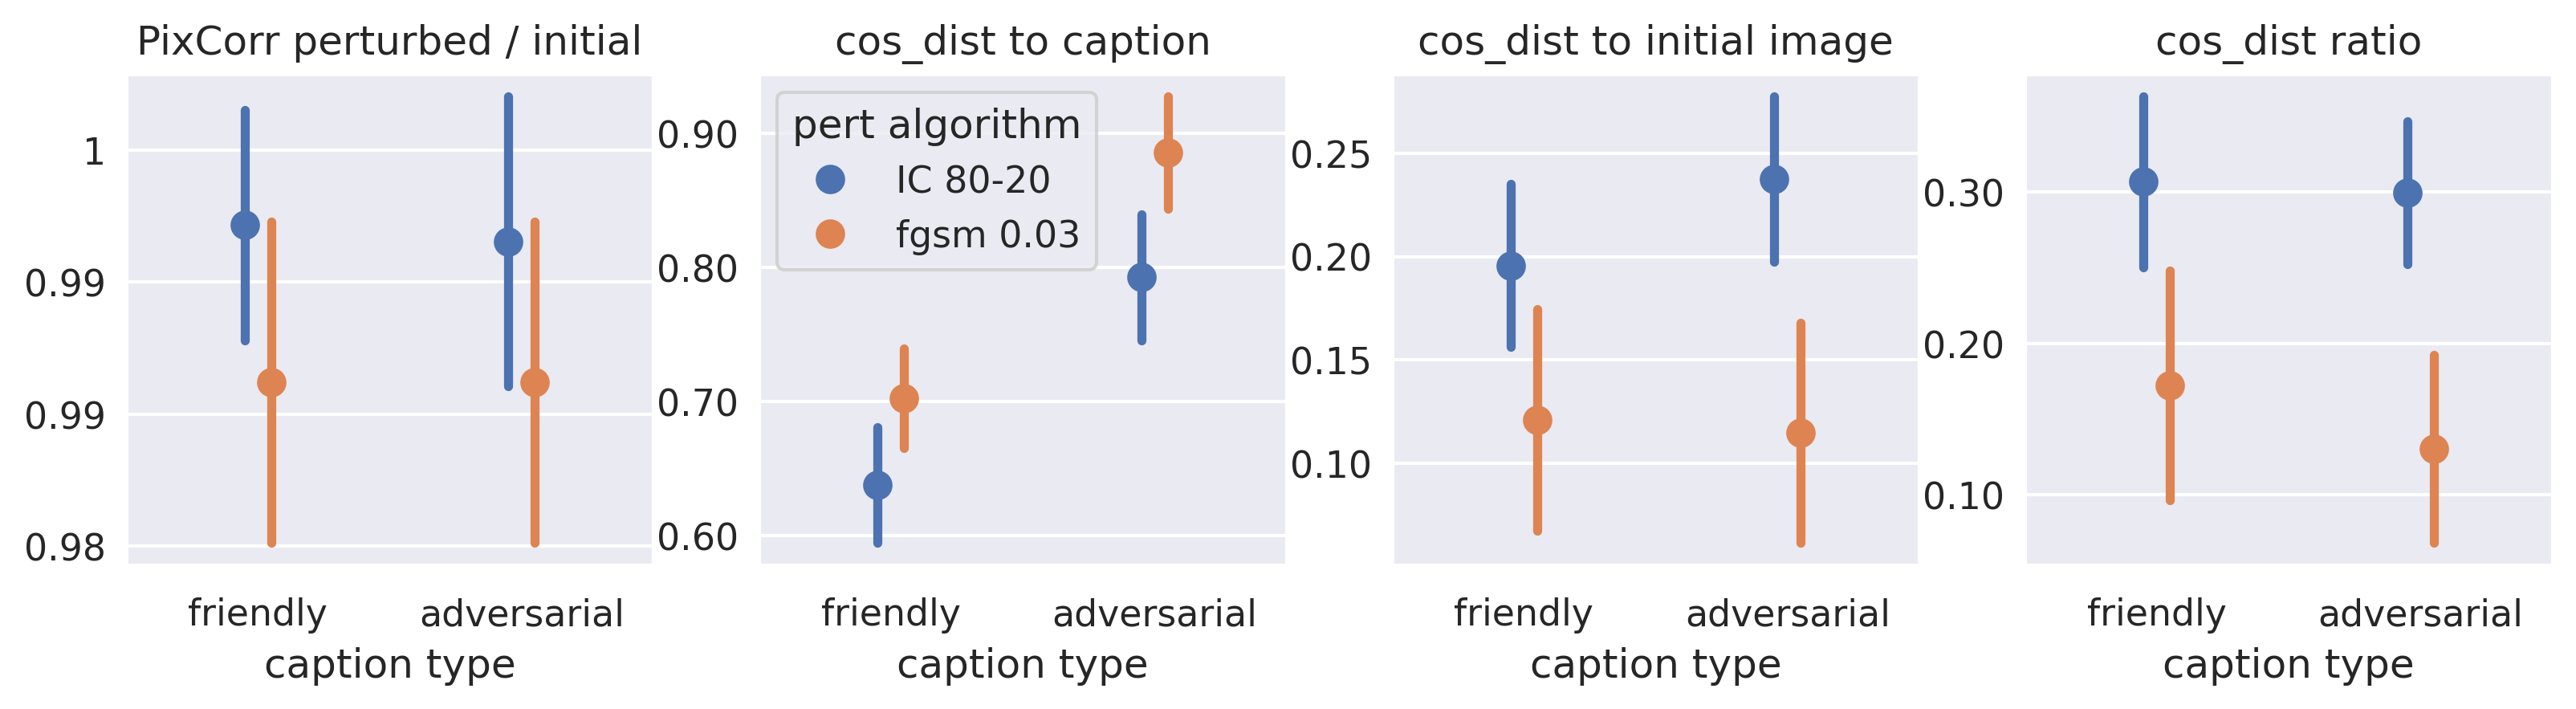
\includegraphics[width=1\textwidth]{plots/advpert_validation_chosen_perts.png}
    \caption{A nice image}\label{fig:advpert_validation_chosen_perts} % TODO: schreiben dass hier SD in den Fehlerbalken ist
\end{figure}
    
For the reconstruction experiments, 5 perturbations were created for each of the 1200 training images with the chosen parameters for IC and fgsm: for the friendly perturbations with all 5 associated captions and for the adversarial perturbations with 5 different randomly selected captions. This results in a total of 6000 training images. The properties of these 6000 images are compared in Figure~\ref{fig:advpert_validation_chosen_perts}. The IC algorithm produces perturbed images that have, on average, a higher pixel correlation than the fgsm algorithm. In addition, both the cosine distance to the desired perturbation vectors is lower and the cosine distance to the original image is slightly higher than for the fgsm algorithm (resulting in a higher cos dist ratio for the IC algorithm than for fgsm). The IC algorithm has thus better achieved the goal of creating perturbations that visually match the fgsm, but can specifically modify the clipvision embeddings.

% Show some of the images qualitatively that will be shown
\begin{figure}[ht]
    \centering
    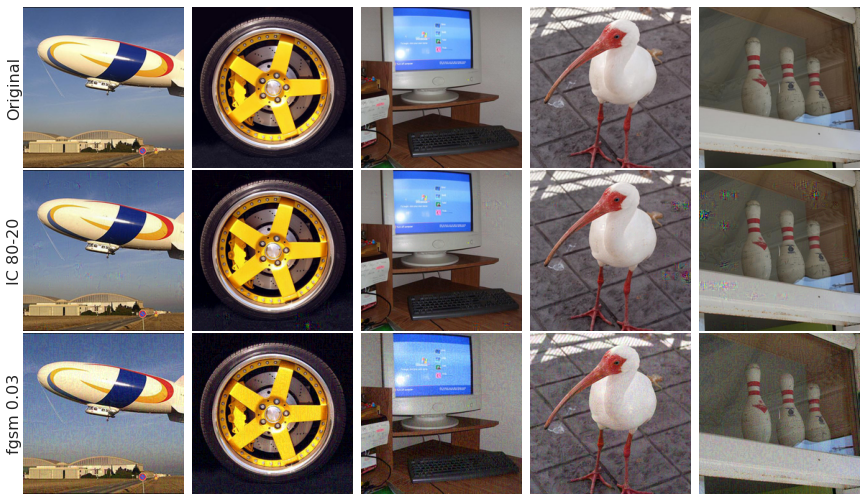
\includegraphics[width=1\textwidth]{plots/advpert_validation_chosen_qual.png}
    \caption{A nice image}\label{fig:advpert_validation_chosen_qual}
\end{figure}

Figure~\ref{fig:advpert_validation_chosen_qual} shows the original and perturbed versions for five images with the two algorithms, as previously shown, the selective artefacts can be seen with IC (particularly visible with the bowling pins) and with fgsm the uniform noise that was superimposed on the image. 


\subsection{Results}

\begin{figure}[ht]
    \centering
    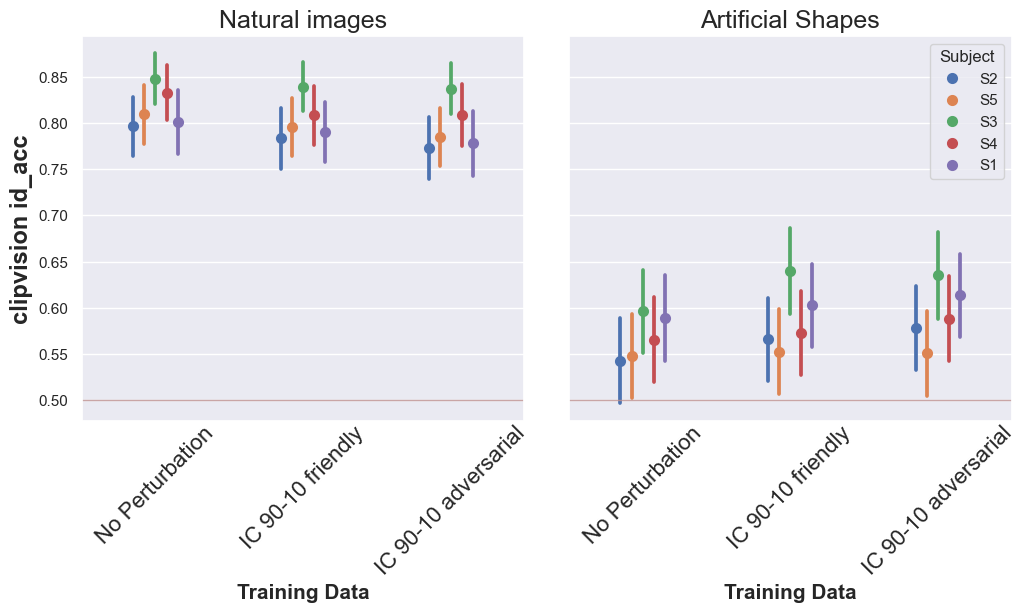
\includegraphics[width=1\textwidth]{plots/advpert_translator_ic_90-10.png}
    \caption{A nice image}\label{fig:advpert_translator_ic_90}
\end{figure}

% \begin{figure}[ht]
%     \centering
%     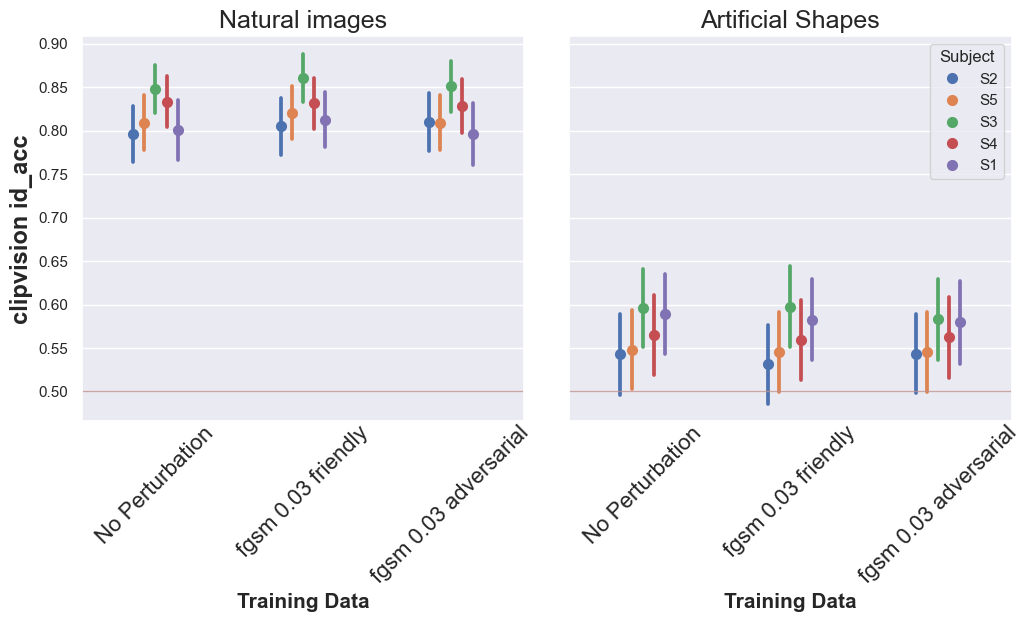
\includegraphics[width=1\textwidth]{plots/advpert_translator_fgsm_0.03.png}
%     \caption{A nice image}\label{fig:advpert_translator_fgsm_0}
% \end{figure}



\begin{figure}[ht]
    \centering
    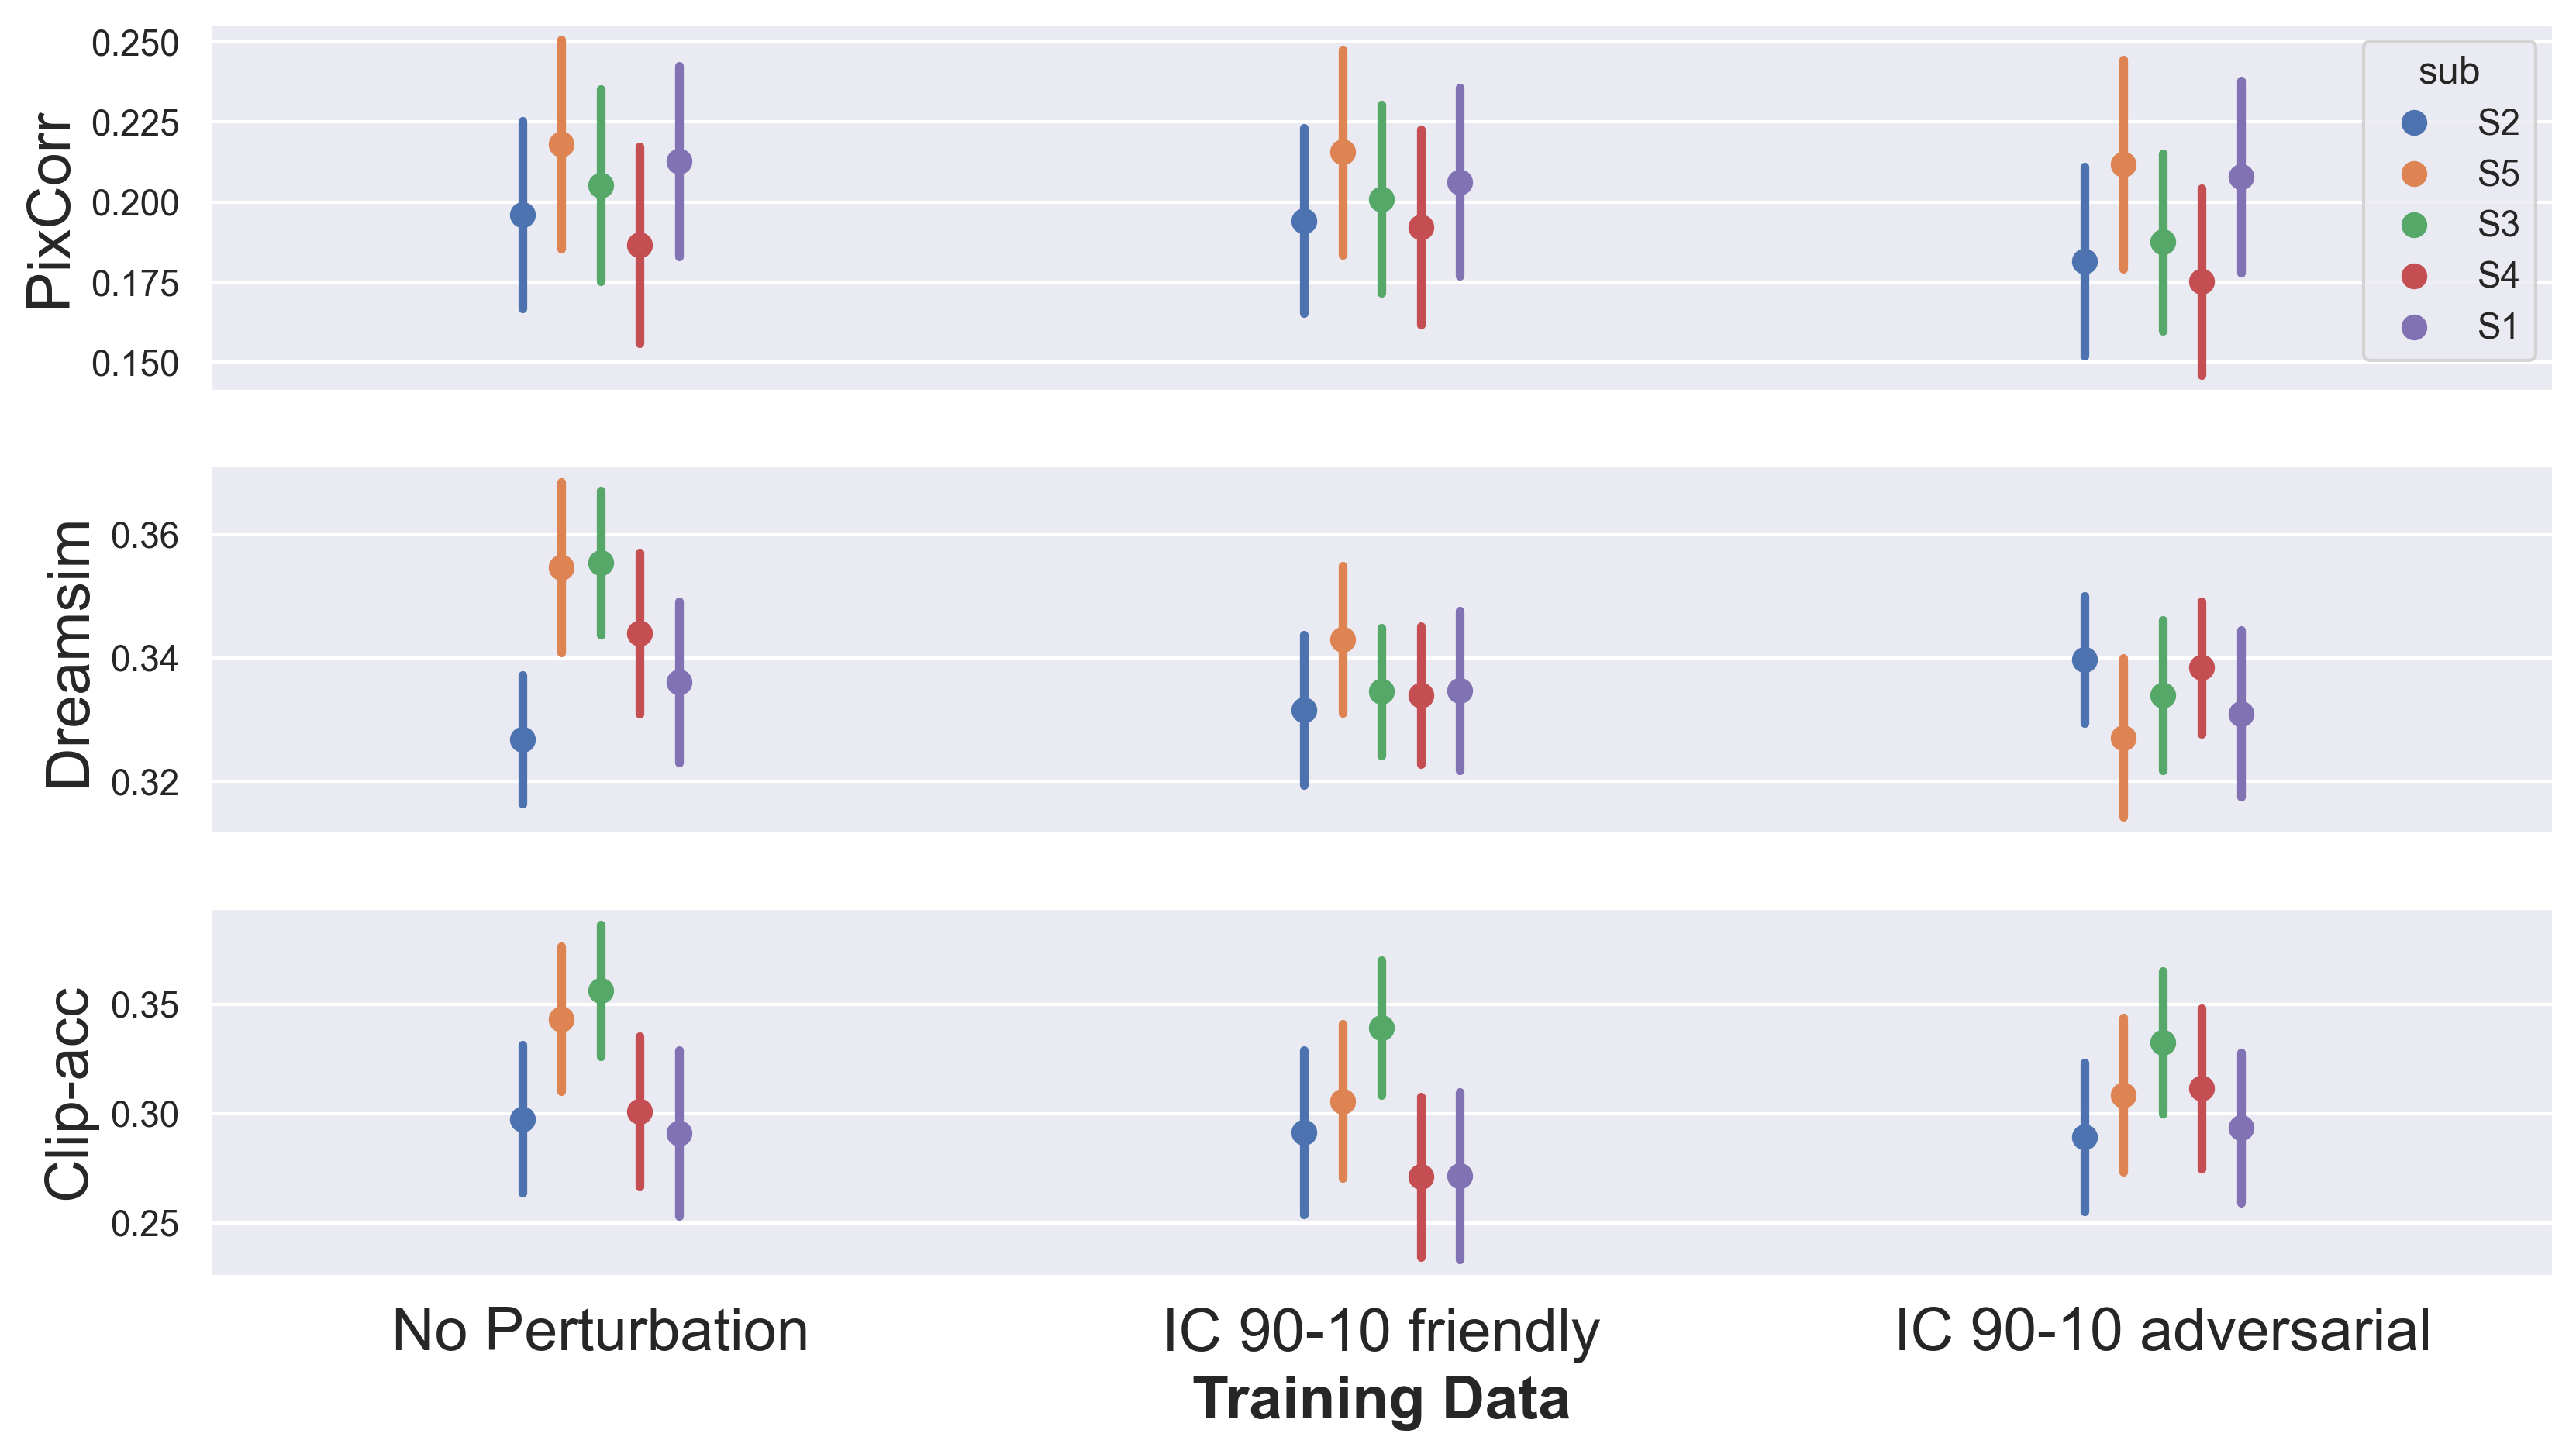
\includegraphics[width=1\textwidth]{plots/advpert_reconstruction_test_ic_90-10.png}
    \caption{A nice image}\label{fig:advpert_reconstruction_test_ic_90}
\end{figure}

\begin{figure}[ht]
    \centering
    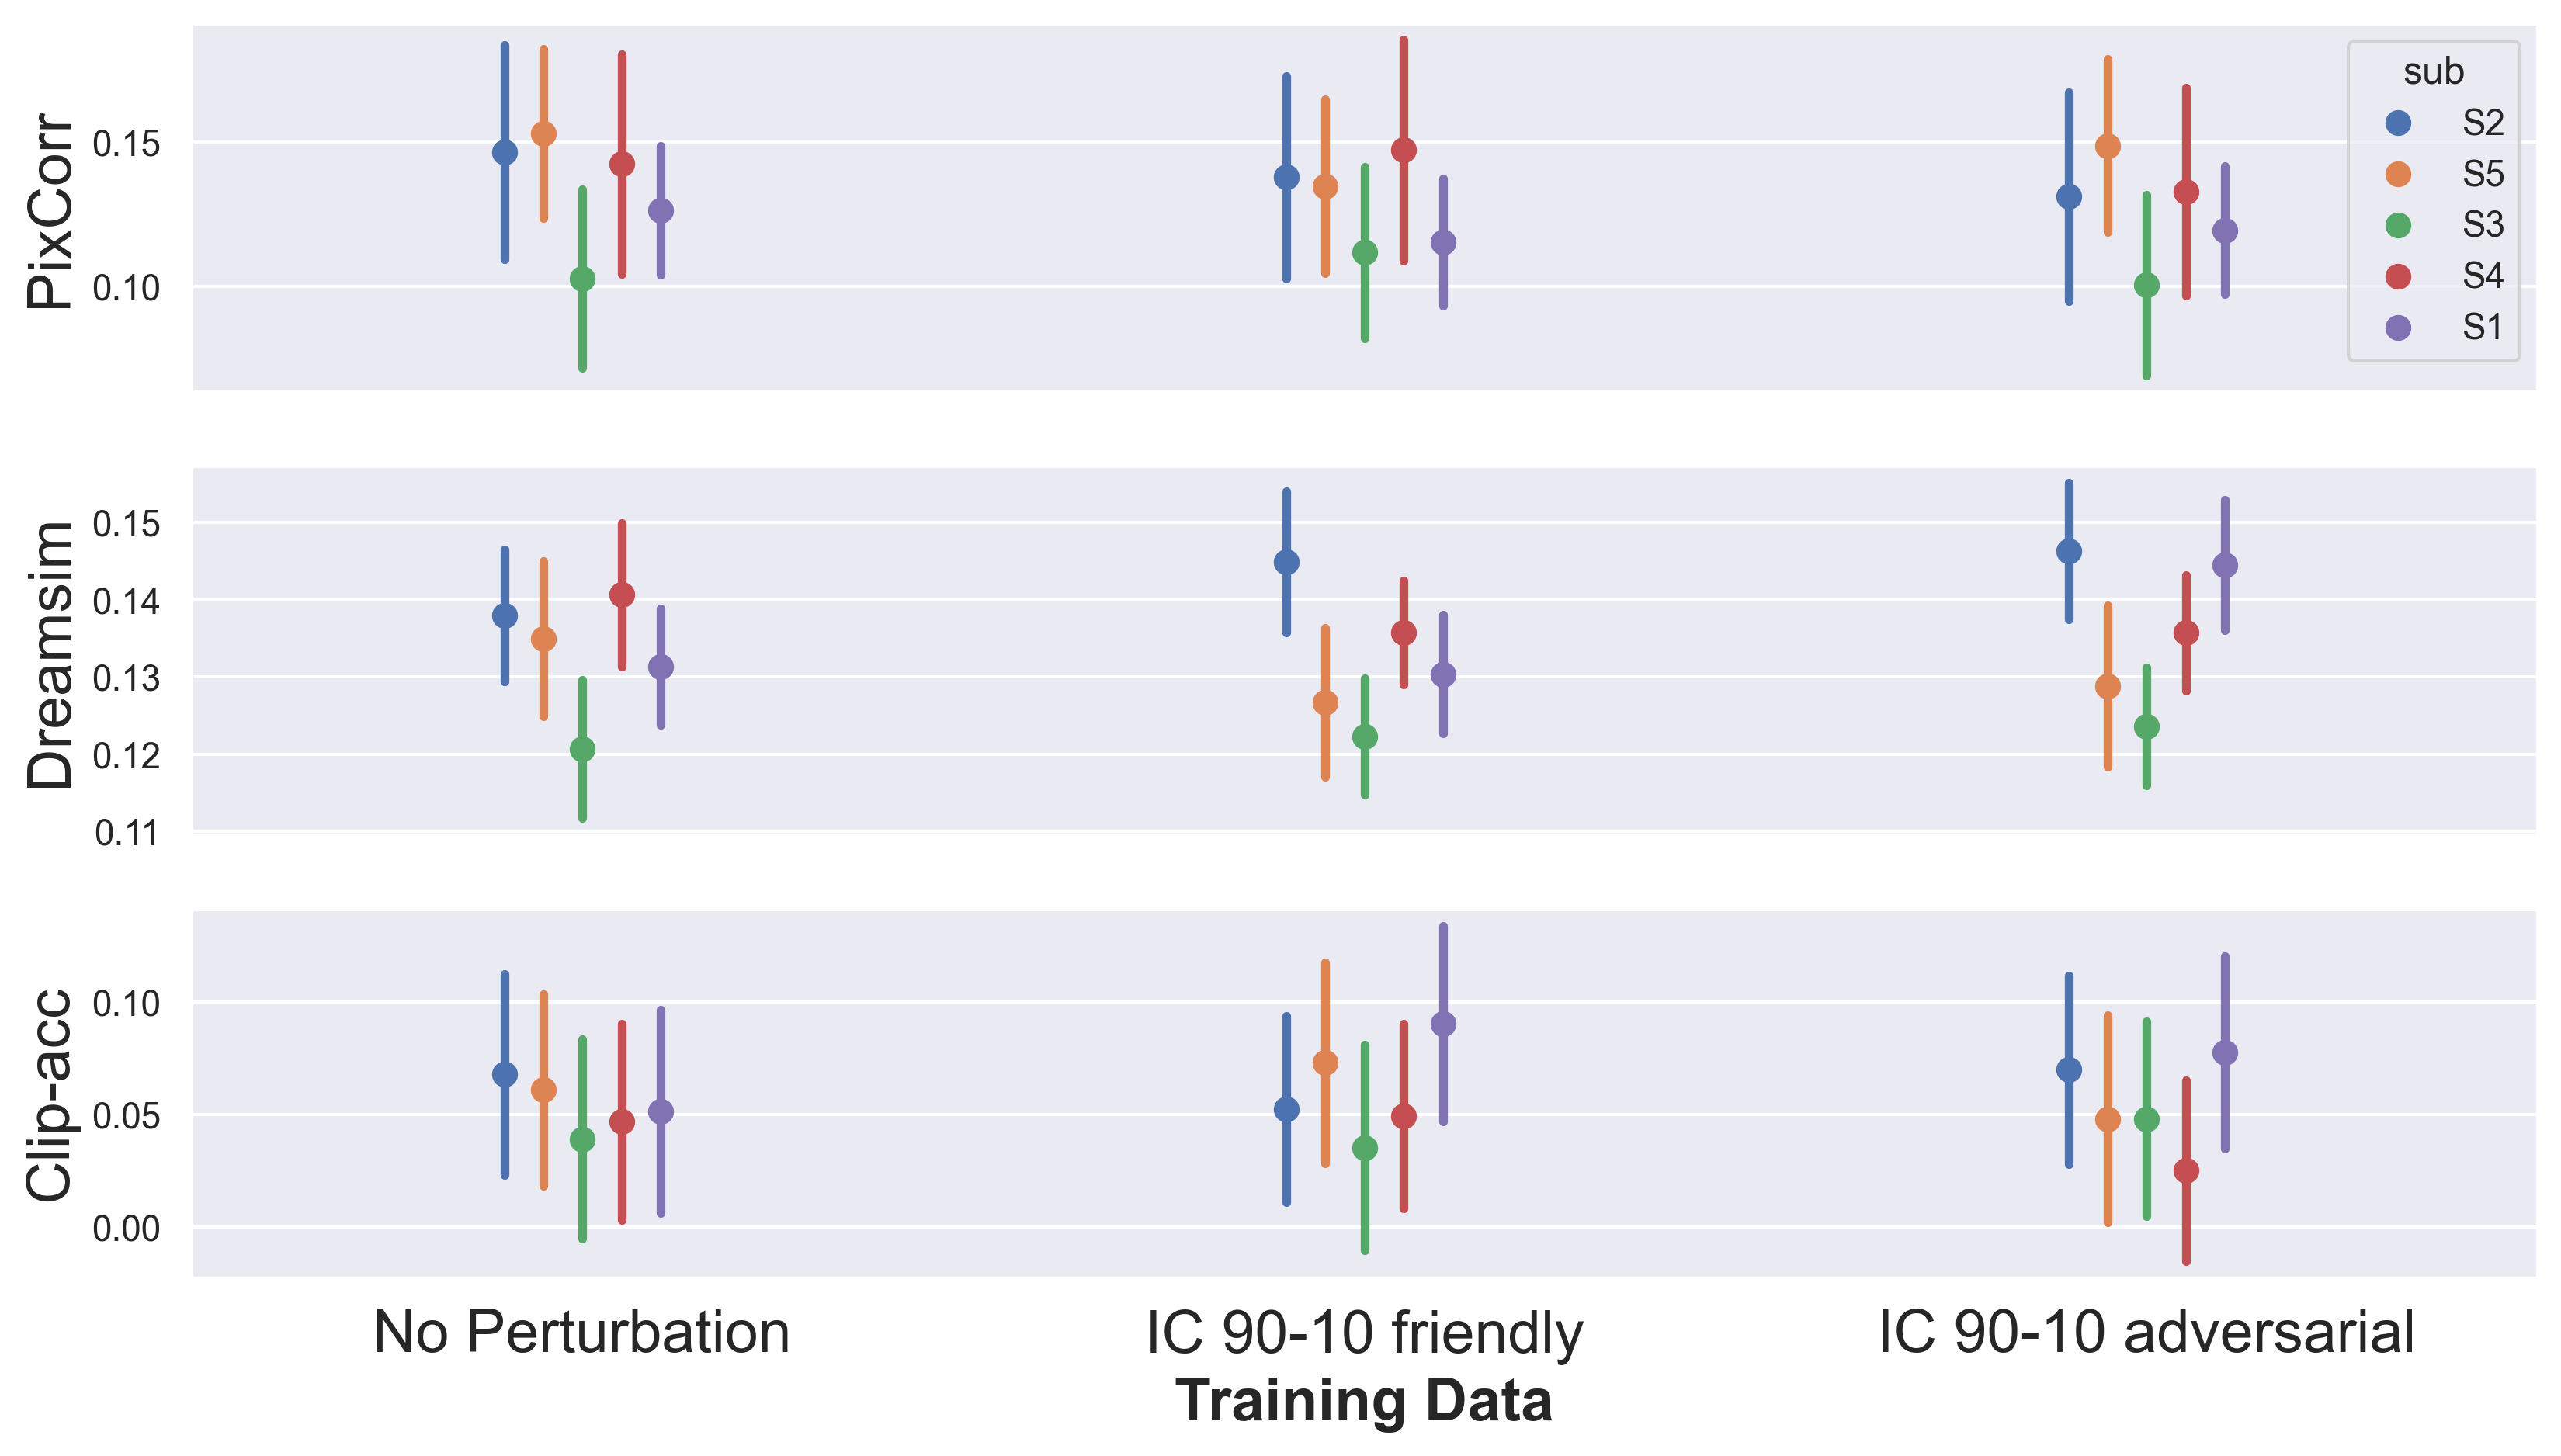
\includegraphics[width=1\textwidth]{plots/advpert_reconstruction_art_ic_90-10.png}
    \caption{A nice image}\label{fig:advpert_reconstruction_art_ic_90}
\end{figure}


% \begin{figure}[ht]
%     \centering
%     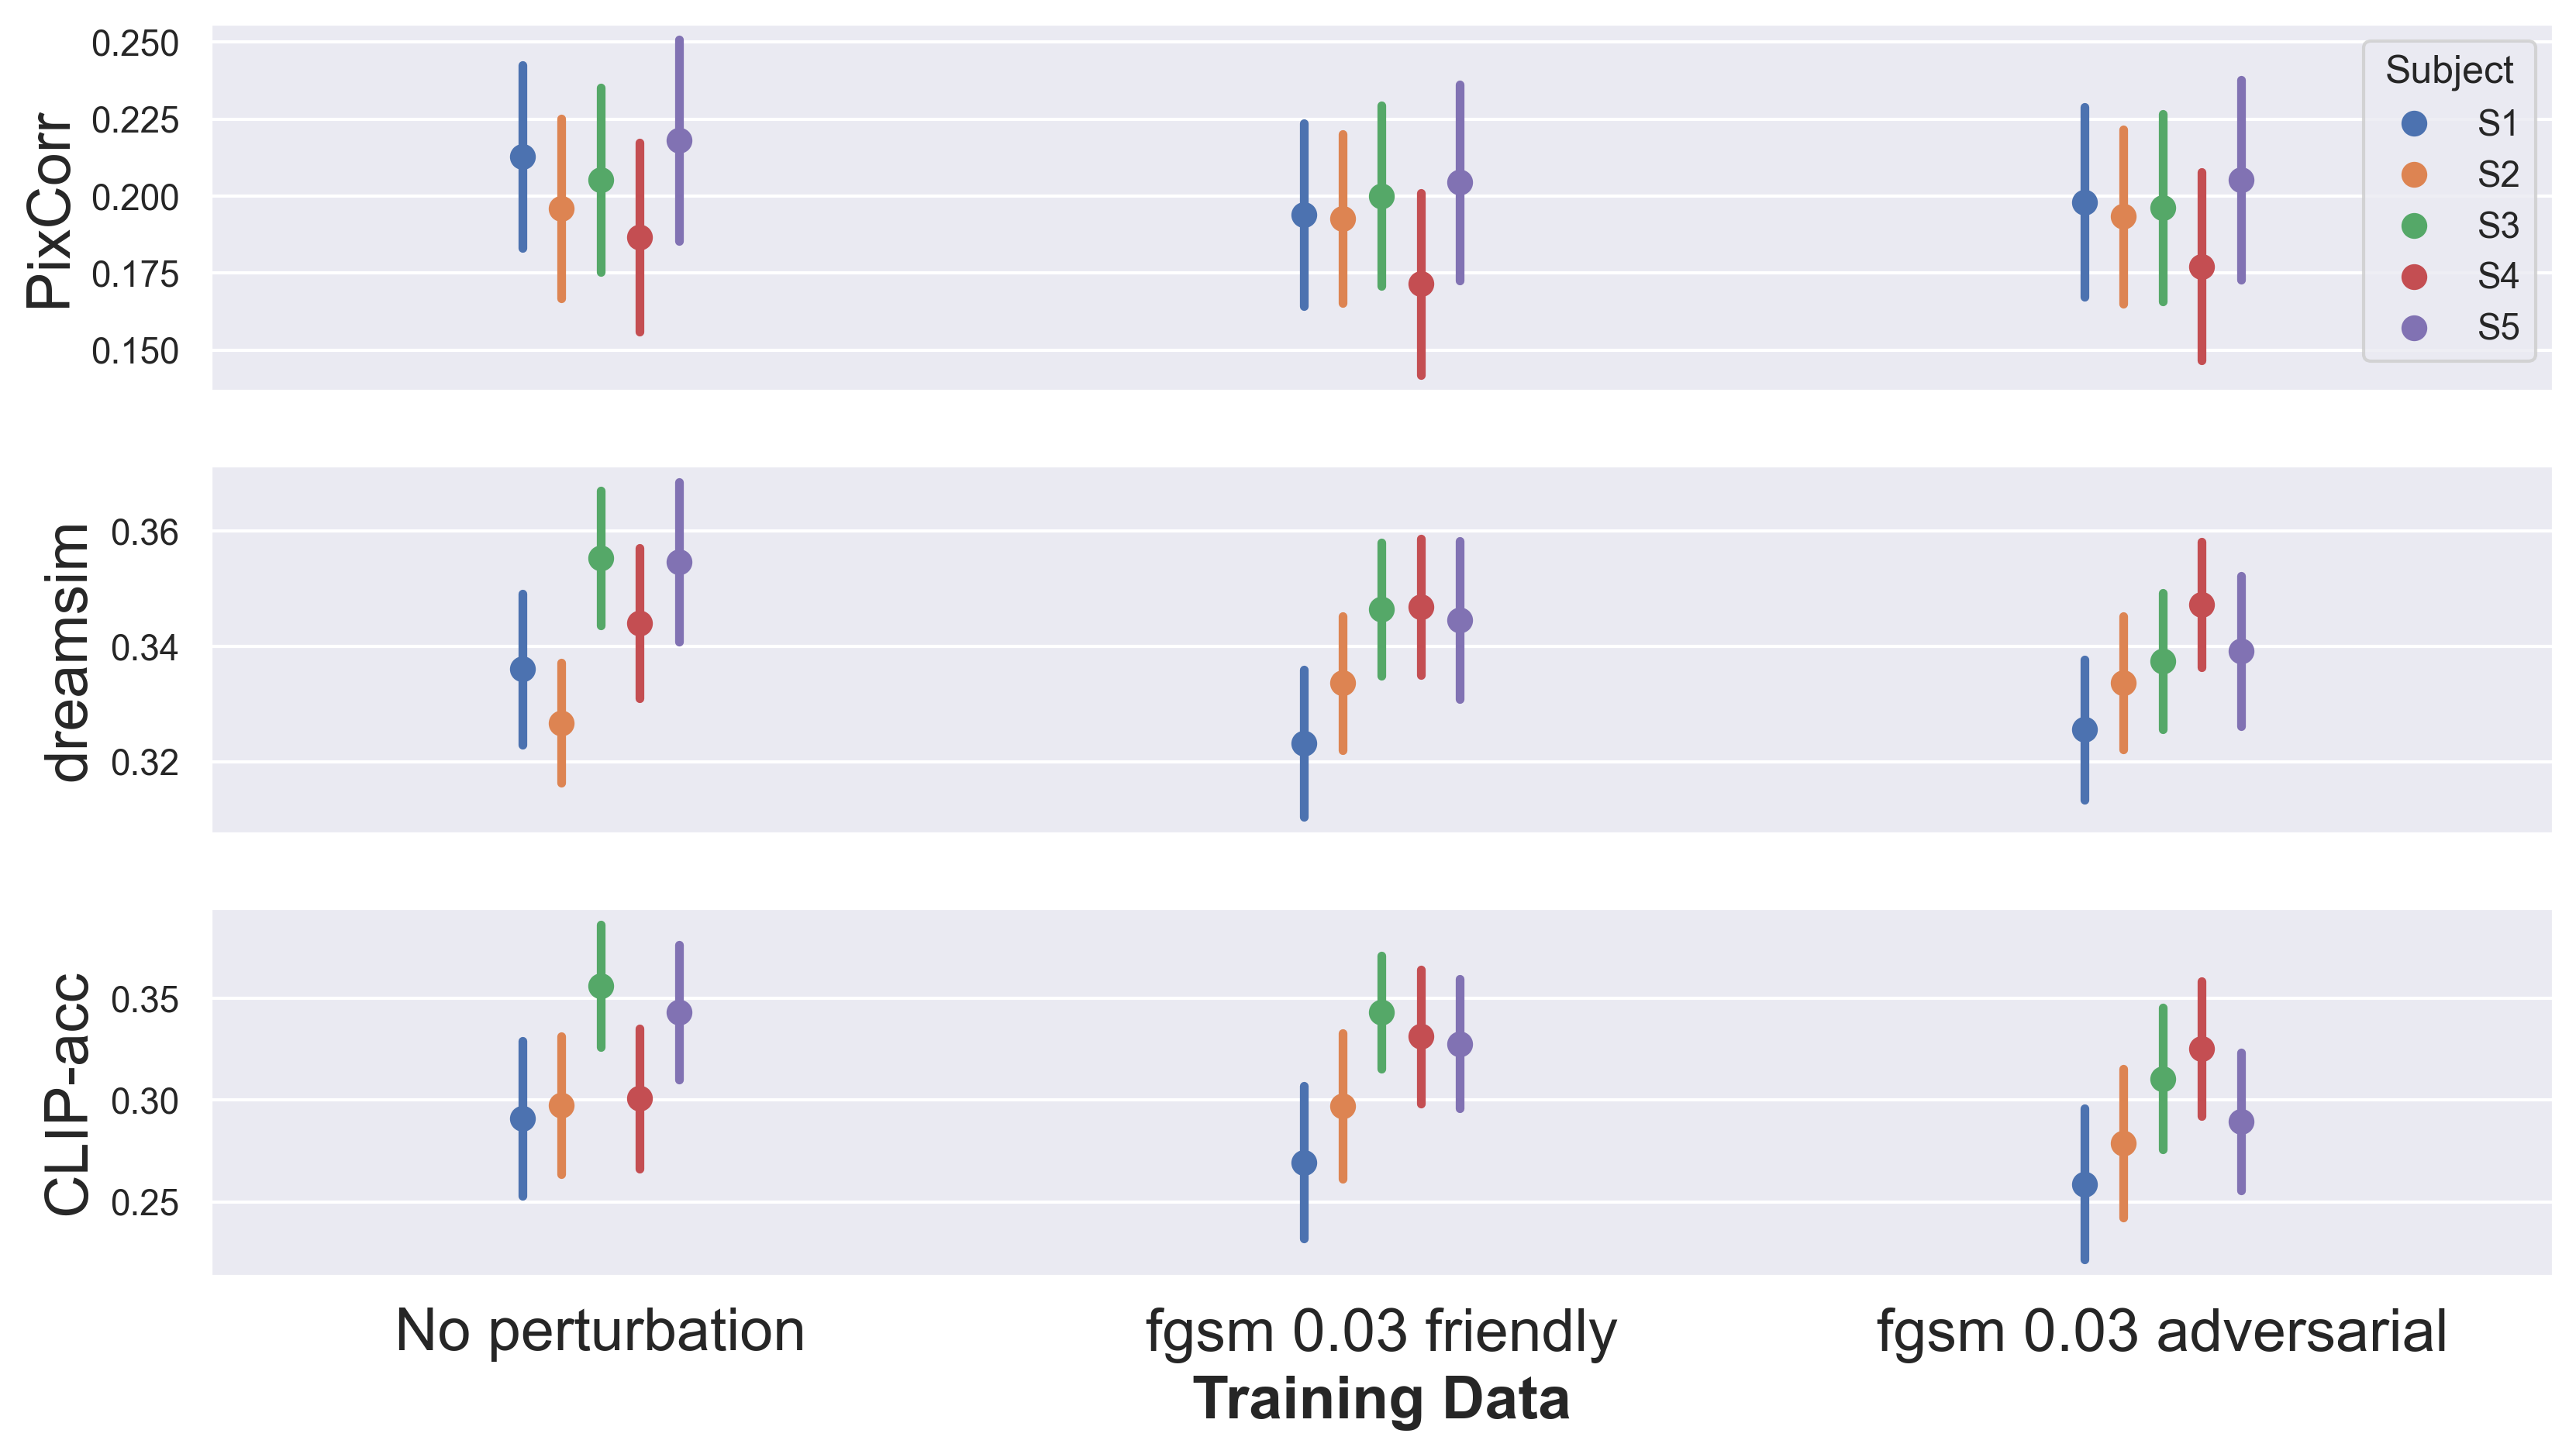
\includegraphics[width=1\textwidth]{plots/advpert_reconstruction_test_fgsm_0.03.png}
%     \caption{A nice image}\label{fig:advpert_reconstruction_test_fgsm_0.03}
% \end{figure}

% \begin{figure}[ht]
%     \centering
%     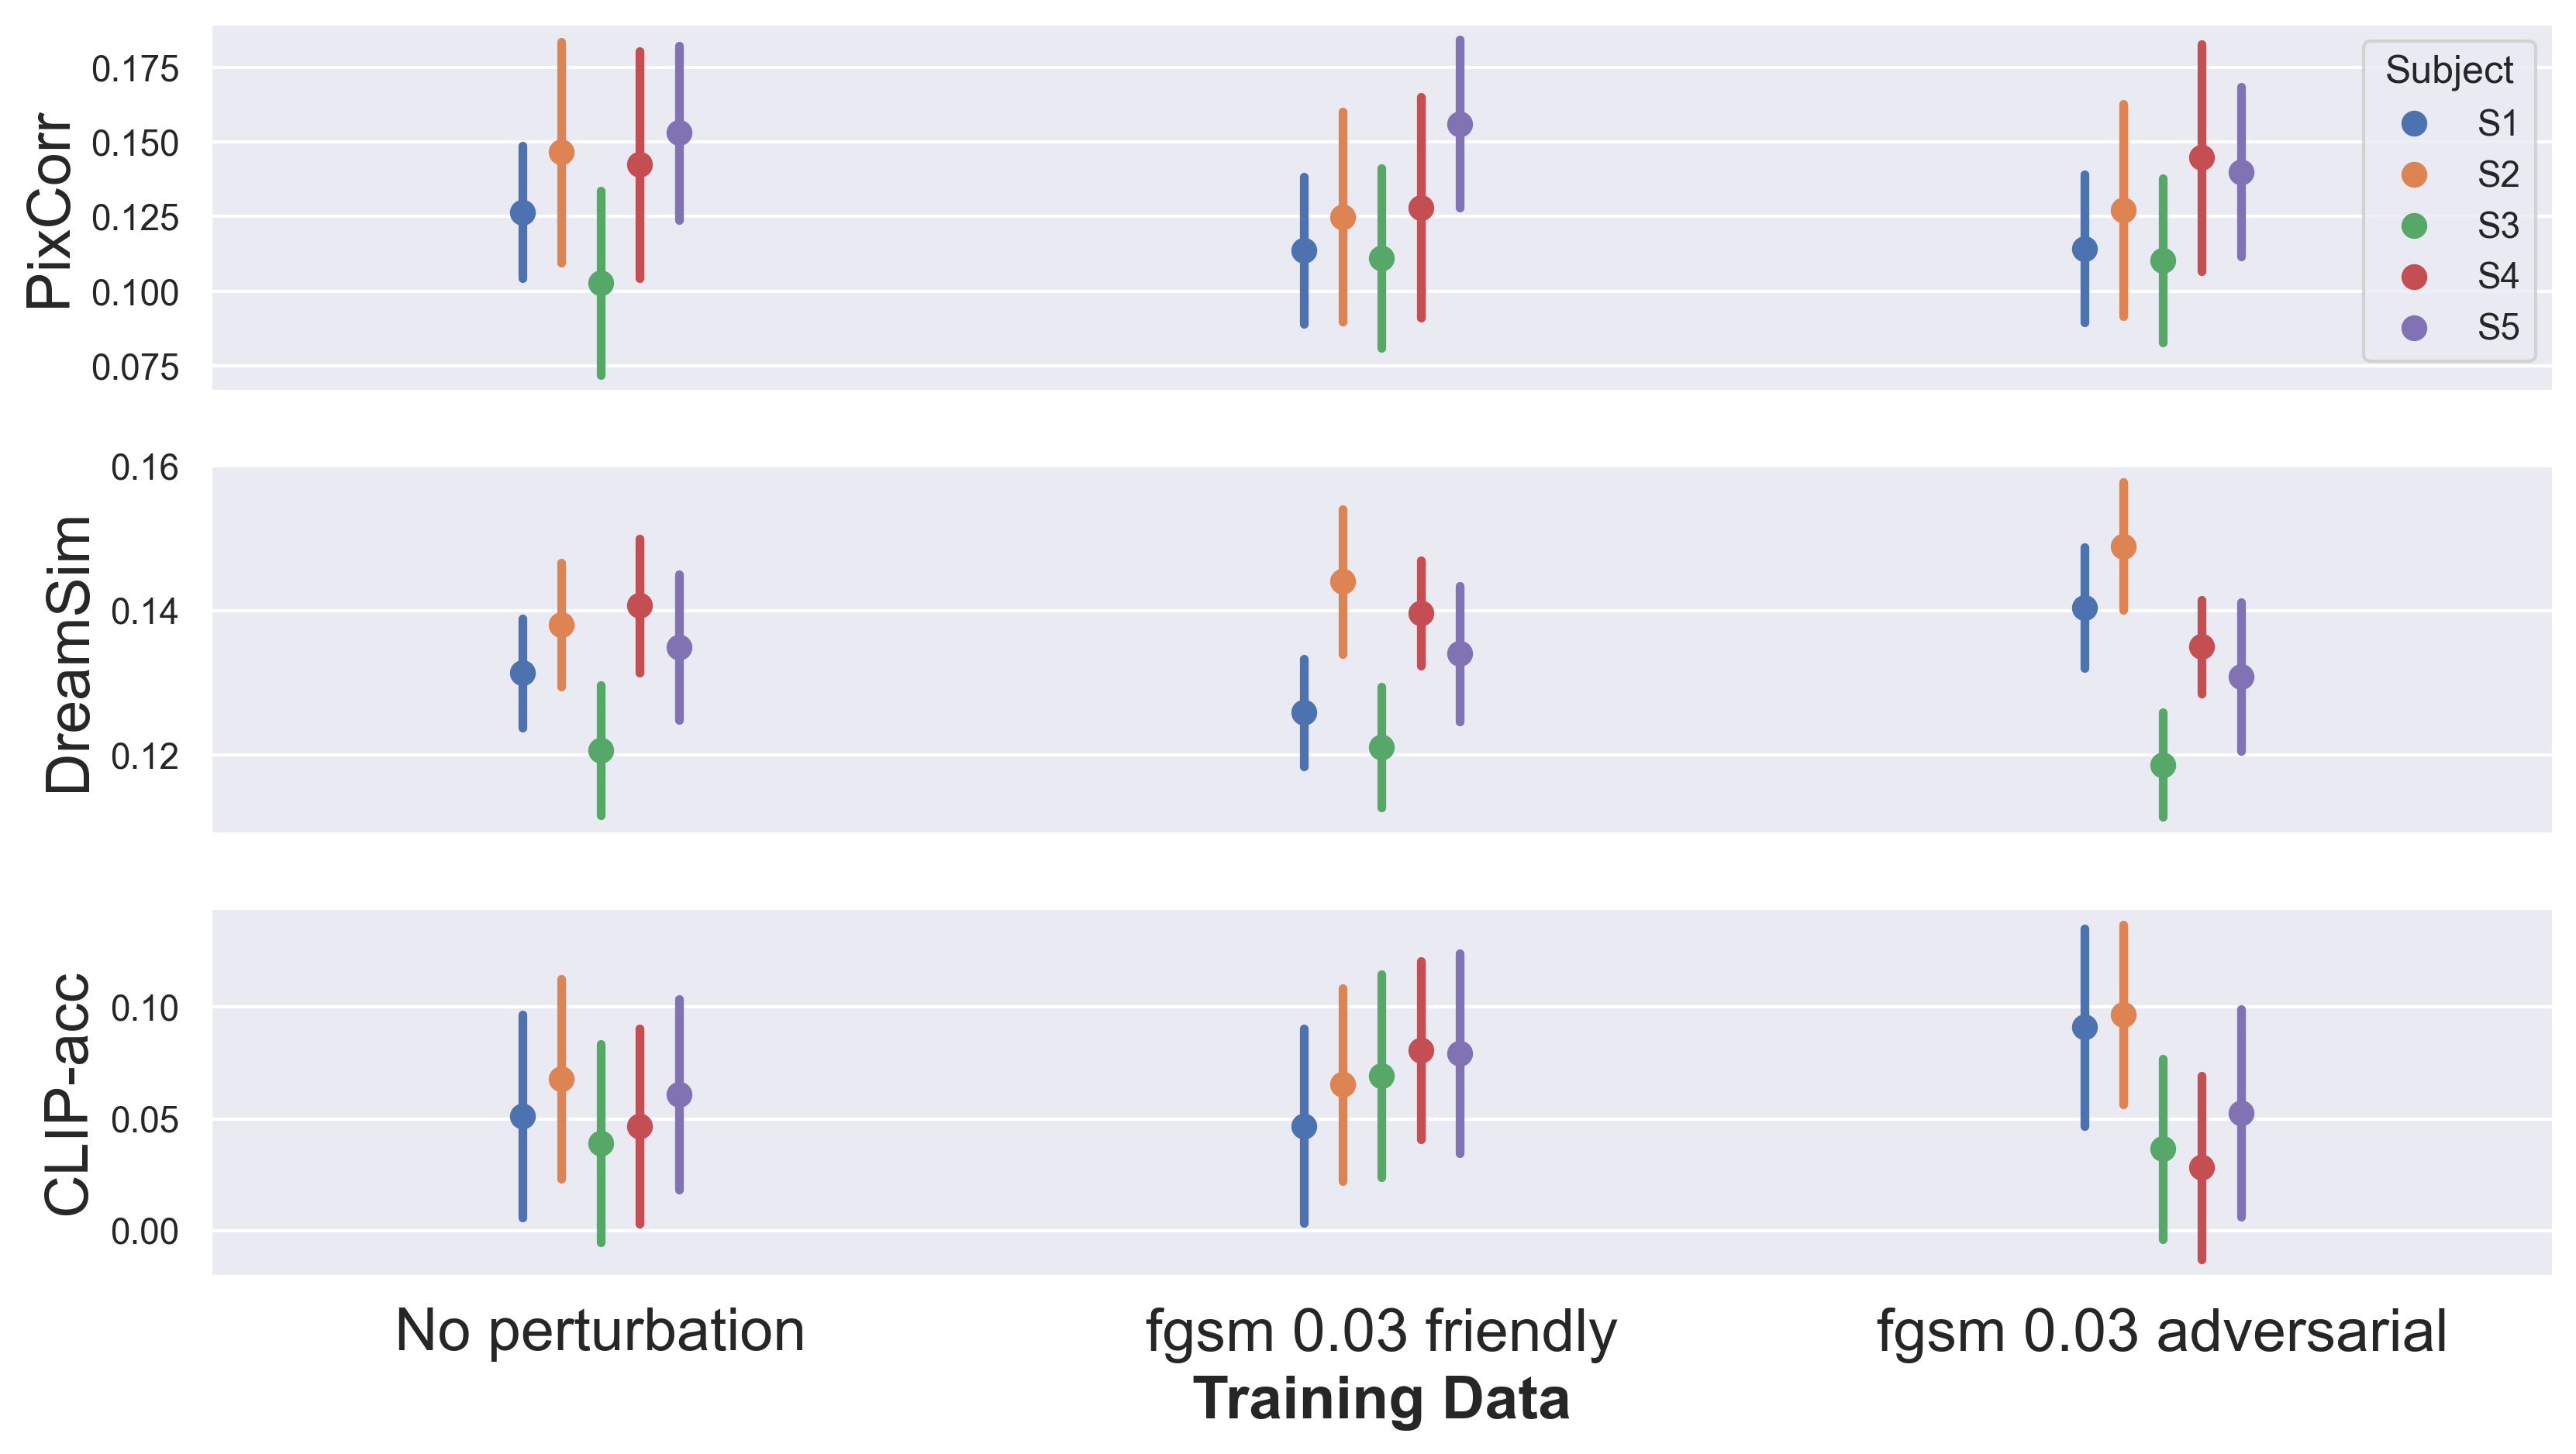
\includegraphics[width=1\textwidth]{plots/advpert_reconstruction_art_fgsm_0.03.png}
%     \caption{A nice image}\label{fig:advpert_reconstruction_art_fgsm_0.03}
% \end{figure}



\subsection{Discussion}

- Das Problem mit der Regression (wir lernen nur den Mittelwert)
- Einschränkung: Man muss natürlich auch sagen, dass menschliche Aufmerksamkeit anders funktioniert, bei einzelnen kleinen Punkten kann ein größerer Unterschied wahrgenommen werden, als bei einem komplette verrauschten Bild
- Man könnte natürlich auch die KI generierten captions genutzen
